%%%%%%%%%%%%%%%%%%%%%%%%%%%%%%%%%%%%%%%%
%% MCM/ICM LaTeX Template %%
%% 2025 MCM/ICM %%
%%%%%%%%%%%%%%%%%%%%%%%%%%%%%%%%%%%%%%%%

% Format
\documentclass[12pt]{article}
\usepackage{geometry}
\geometry{left=1in, right=0.75in, top=1in, bottom=1in}

\newcommand{\Problem}{F}
\newcommand{\Team}{2500434}

\usepackage{newtxtext}
\usepackage{amsmath,amssymb,amsthm}
\usepackage{newtxmath}
\usepackage[pdftex]{graphicx}
\usepackage{subfig}
\usepackage{xcolor}
\usepackage{fancyhdr}
\usepackage{enumitem}
\usepackage{titlesec}
\usepackage{tocloft}
\usepackage{lastpage}

% Page Settings
\pagestyle{fancy}
\lhead{Team \# \Team}
\rhead{Page \thepage\ of \pageref{LastPage}}

% Mathematical env.
\newtheorem{theorem}{Theorem}
\newtheorem{corollary}[theorem]{Corollary}
\newtheorem{lemma}[theorem]{Lemma}
\newtheorem{definition}{Definition}

% Format of table of contents
\renewcommand{\cftsecleader}{\cftdotfill{\cftdotsep}}
\renewcommand{\contentsname}{\begin{center} INDEX \end{center}}

% Format of subsection and subsubsection
\titleformat{\section}{\bfseries\raggedright\Large}{\thesection}{1em}{}
\titleformat{\subsection}{\bfseries\raggedright}{\thesubsection}{1em}{}{}
\titleformat{\subsubsection}{\bfseries}{\hspace*{2em}\thesubsubsection}{1em}{}{}

% CoverPage Design
\begin{document}
\graphicspath{{.}}  % Place the graphic file in the same directory as the main document
\DeclareGraphicsExtensions{.pdf, .jpg, .tif, .png}
\thispagestyle{empty}
\vspace*{-16ex}
\centerline{
\begin{tabular}{*3{c}}
	\parbox[t]{0.3\linewidth}{\begin{center}\textbf{Problem Chosen}\\ \Large \textcolor{red}{\Problem}\end{center}}
	& \parbox[t]{0.3\linewidth}{\begin{center}\textbf{2025\\ MCM/ICM\\ Summary Sheet}\end{center}}
	& \parbox[t]{0.3\linewidth}{\begin{center}\textbf{Team Control Number}\\ \Large \textcolor{red}{\Team}\end{center}}	\\
	\hline
\end{tabular}}

% TODO: Summary
% 1. 12-point Times New Roman font ;
% 2. pdf naming format: 2500434.pdf ;
% 3. No name of school, advisor, or team members .
\begin{center}
Hello Summary!
\end{center}

\newpage
\tableofcontents
\newpage

\section{Introduction}\label{sec:introduction} %1
	\subsection{Background}\label{subsec:background} %1.1
		In the digital age, the speed and scale of global connectivity have reached unprecedented heights.
		However, with technological advancements, \textbf{cybercrime} has also become increasingly complex and diverse.
		These crimes pose significant threats and challenges to personal privacy, corporate assets, national security, and social stability.
		The transnational and covert nature of cybercrime makes it difficult to address effectively.
		Attackers often exploit legal differences and technical vulnerabilities across countries to evade accountability.
		Additionally, many businesses and institutions, concerned about their reputation and commercial interests,
		often choose \textbf{not to publicly report} cyberattacks, opting instead to pay ransoms or handle incidents privately.
		This further exacerbates the hidden nature of cybercrime.
		Developed countries, with their highly digitized economic and social structures, are often prime targets for cybercrime, while
		developing countries face their own unique challenges.

		To address this global challenge, countries have introduced national cybersecurity \textbf{policies}
		aimed at enhancing their defensive capabilities through legal, technical, and organizational cooperation.
		The \textbf{effectiveness} of these policies varies significantly across nations, and these differences may be closely related to factors
		such as policy design, enforcement, technological infrastructure, education levels, economic development, and internet penetration rates.
		In this context, understanding which factors make certain countries' cybersecurity policies more effective has become a critical issue.
		By analyzing the global distribution of cybercrime, national cybersecurity policies, and their outcomes,
		we can identify which policies and laws are particularly effective in preventing, prosecuting, and mitigating cybercrime.
		This data-driven analysis not only helps countries improve their cybersecurity policies
		but also provides valuable insights for global cybersecurity cooperation.
	\subsection{Restatement of the problem}\label{subsec:restatement-of-the-problem} %1.2
		We are required to identify patterns
		that can inform the data-driven development and refinement of national cybersecurity policies and laws,
		which focused on those that have demonstrated effectiveness.
		Our goal is to develop a theory explaining what constitutes a strong national cybersecurity policy and then
		support it with a data-driven analysis.

		Several key aspects are listed below:
		\begin{itemize}
			\item Patterns in cybercrime distributed worldwide.
			\item Assessment to effectiveness of National Cybersecurity Policies.
			\item Correlation between national demographics and our distribution analysis.
		\end{itemize}
	\subsection{Analysis of problems}\label{subsec:analysis-of-problems} %1.3
		We have divided each problem into several different steps:
		\subsubsection[]{Cybercrime distribution across the world} %1.3.1
			\begin{itemize}
				\item Process the JSON files published on VCDB .
				\item Use GCI as the primary indicator to assess countries with disproportionately high levels of cybercrime.
				\item Group countries based on GCI Tier measure, and
					visually represent the distribution of cybercrime in each group using heatmaps.
			\end{itemize}
		\subsubsection[]{Effective policy or law analytical approach} %1.3.2
			\begin{itemize}
				\item Identify a representative country from each of the T1 to T5 national clusters and
					collect cybersecurity-related policies enacted by these countries.
				\item Plot time-series line graphs depicting the trends of cybercrime over time and
					analyze which policies have been effective in curbing criminal activities.
				\item Conduct a targeted analysis of specific policy models' effectiveness in certain countries,
					focusing on particular indicators.
				\item Integrate temporal factors and national contexts to comprehensively evaluate the impact of policies.
			\end{itemize}
		\subsubsection[]{National demographics correlation} %1.3.3
			\begin{itemize}
				\item TODO % TODO: fill the blank 1.3.3
			\end{itemize}

\section{Symbol and Assumptions}\label{sec:symbol-and-assumptions} %2
	\subsection{Symbol Description}\label{subsec:symbol-description} %2.1
		\begin{tabular}{ll}
			\textbf{Symbol} & \textbf{Description} \\
			\hline
			$D_i$ & Cybercrime distribution in each country \\
			\hline
			$P_i$ & Population of each country \\
			\hline
			$y$   & Transformed value using \( y = \log(1 + x) \). \\
			\hline
		\end{tabular}

		\medskip

		\noindent
		\begin{tabular}{ll}
			\textbf{Abbreviation} & \textbf{Full Form} \\
			\hline
			GCI   & Global Cybersecurity Index\cite{gci-2024} \\
			\hline
			VERIS & the Vocabulary for Event Recording and Incident Sharing\cite{veris} \\
			\hline
			VCDB  & the VERIS Community Database\cite{vcdb} \\
			\hline
		\end{tabular}
	\subsection{Assumption}\label{subsec:assumption} %2.2
		\begin{itemize}
			\item Countries with a population below 5\% are excluded from the consideration of cybercrime distribution because
				a small change of number could bring a significant difference to statistical analysis.
			\item In the statistical analysis of the global distribution of cybercrime,
				factors such as national population growth, internet access, wealth levels, and education levels
				are assumed to have no significant impact on the quantitative distribution of cybercrime incidents.
				This study hypothesizes that the distribution of cybercrime can be more intuitively understood by focusing solely on the number of incidents,
				independent of these socio-economic variables.
				This assumption is based on all available data recorded since the inception of cybercrime statistics,
				aiming to isolate the distribution patterns of cybercrime from other potential influencing factors.
		\end{itemize}

\section{A Data-Driven Model for Global Cybercrime Hotspot Mapping}\label{sec:a-data-driven-model-for-global-cybercrime-hotspot-mapping}
Despite the continuous evolution of national cybercrime since the inception of data collection,
along with changes in policies, legal frameworks, and population demographics,
we can create a global cybercrime hotspot map by leveraging crime data recorded by VERIS over the years.
This not only facilitates the analysis of cybercrime volumes by country
but also allows for fitting the data against policy and population variables to assess their influence on cybercrime trends.
\subsection{Cybercrime distribution across the globe}\label{subsec:Building-the-hotspot-map} %3.1
	We made use of a world-wide map to represent all cybercrime occurred around the world.
	In the map, the color filled in each country represents the total number of cybercrime incidents recorded since the beginning of the statistics.
	The color gradient, ranging from dark blue to dark red, corresponds to eight severity levels (1 to 8).
	Countries marked in blue indicate a low frequency of cybercrime incidents, while those marked in red represent a high density of such incidents.
	For instance, the United States, where the VERIS concept was first proposed, has the highest number of recorded incidents (7,236),
	whereas many other countries have only 1 or 2 recorded incidents.
	To address this significant disparity in data distribution, we applied a logarithmic transformation to the data using the formula
	\[ y=\log(1+x) \]
	where x here represents $D_i$.
	This transformation was implemented using the function
	\[ np.log1p() \]
	in Python to ensure computational precision and stability, particularly for small values.
	The final results are visualized in Figure 1.
	\begin{figure}[htbp]
		\centering
		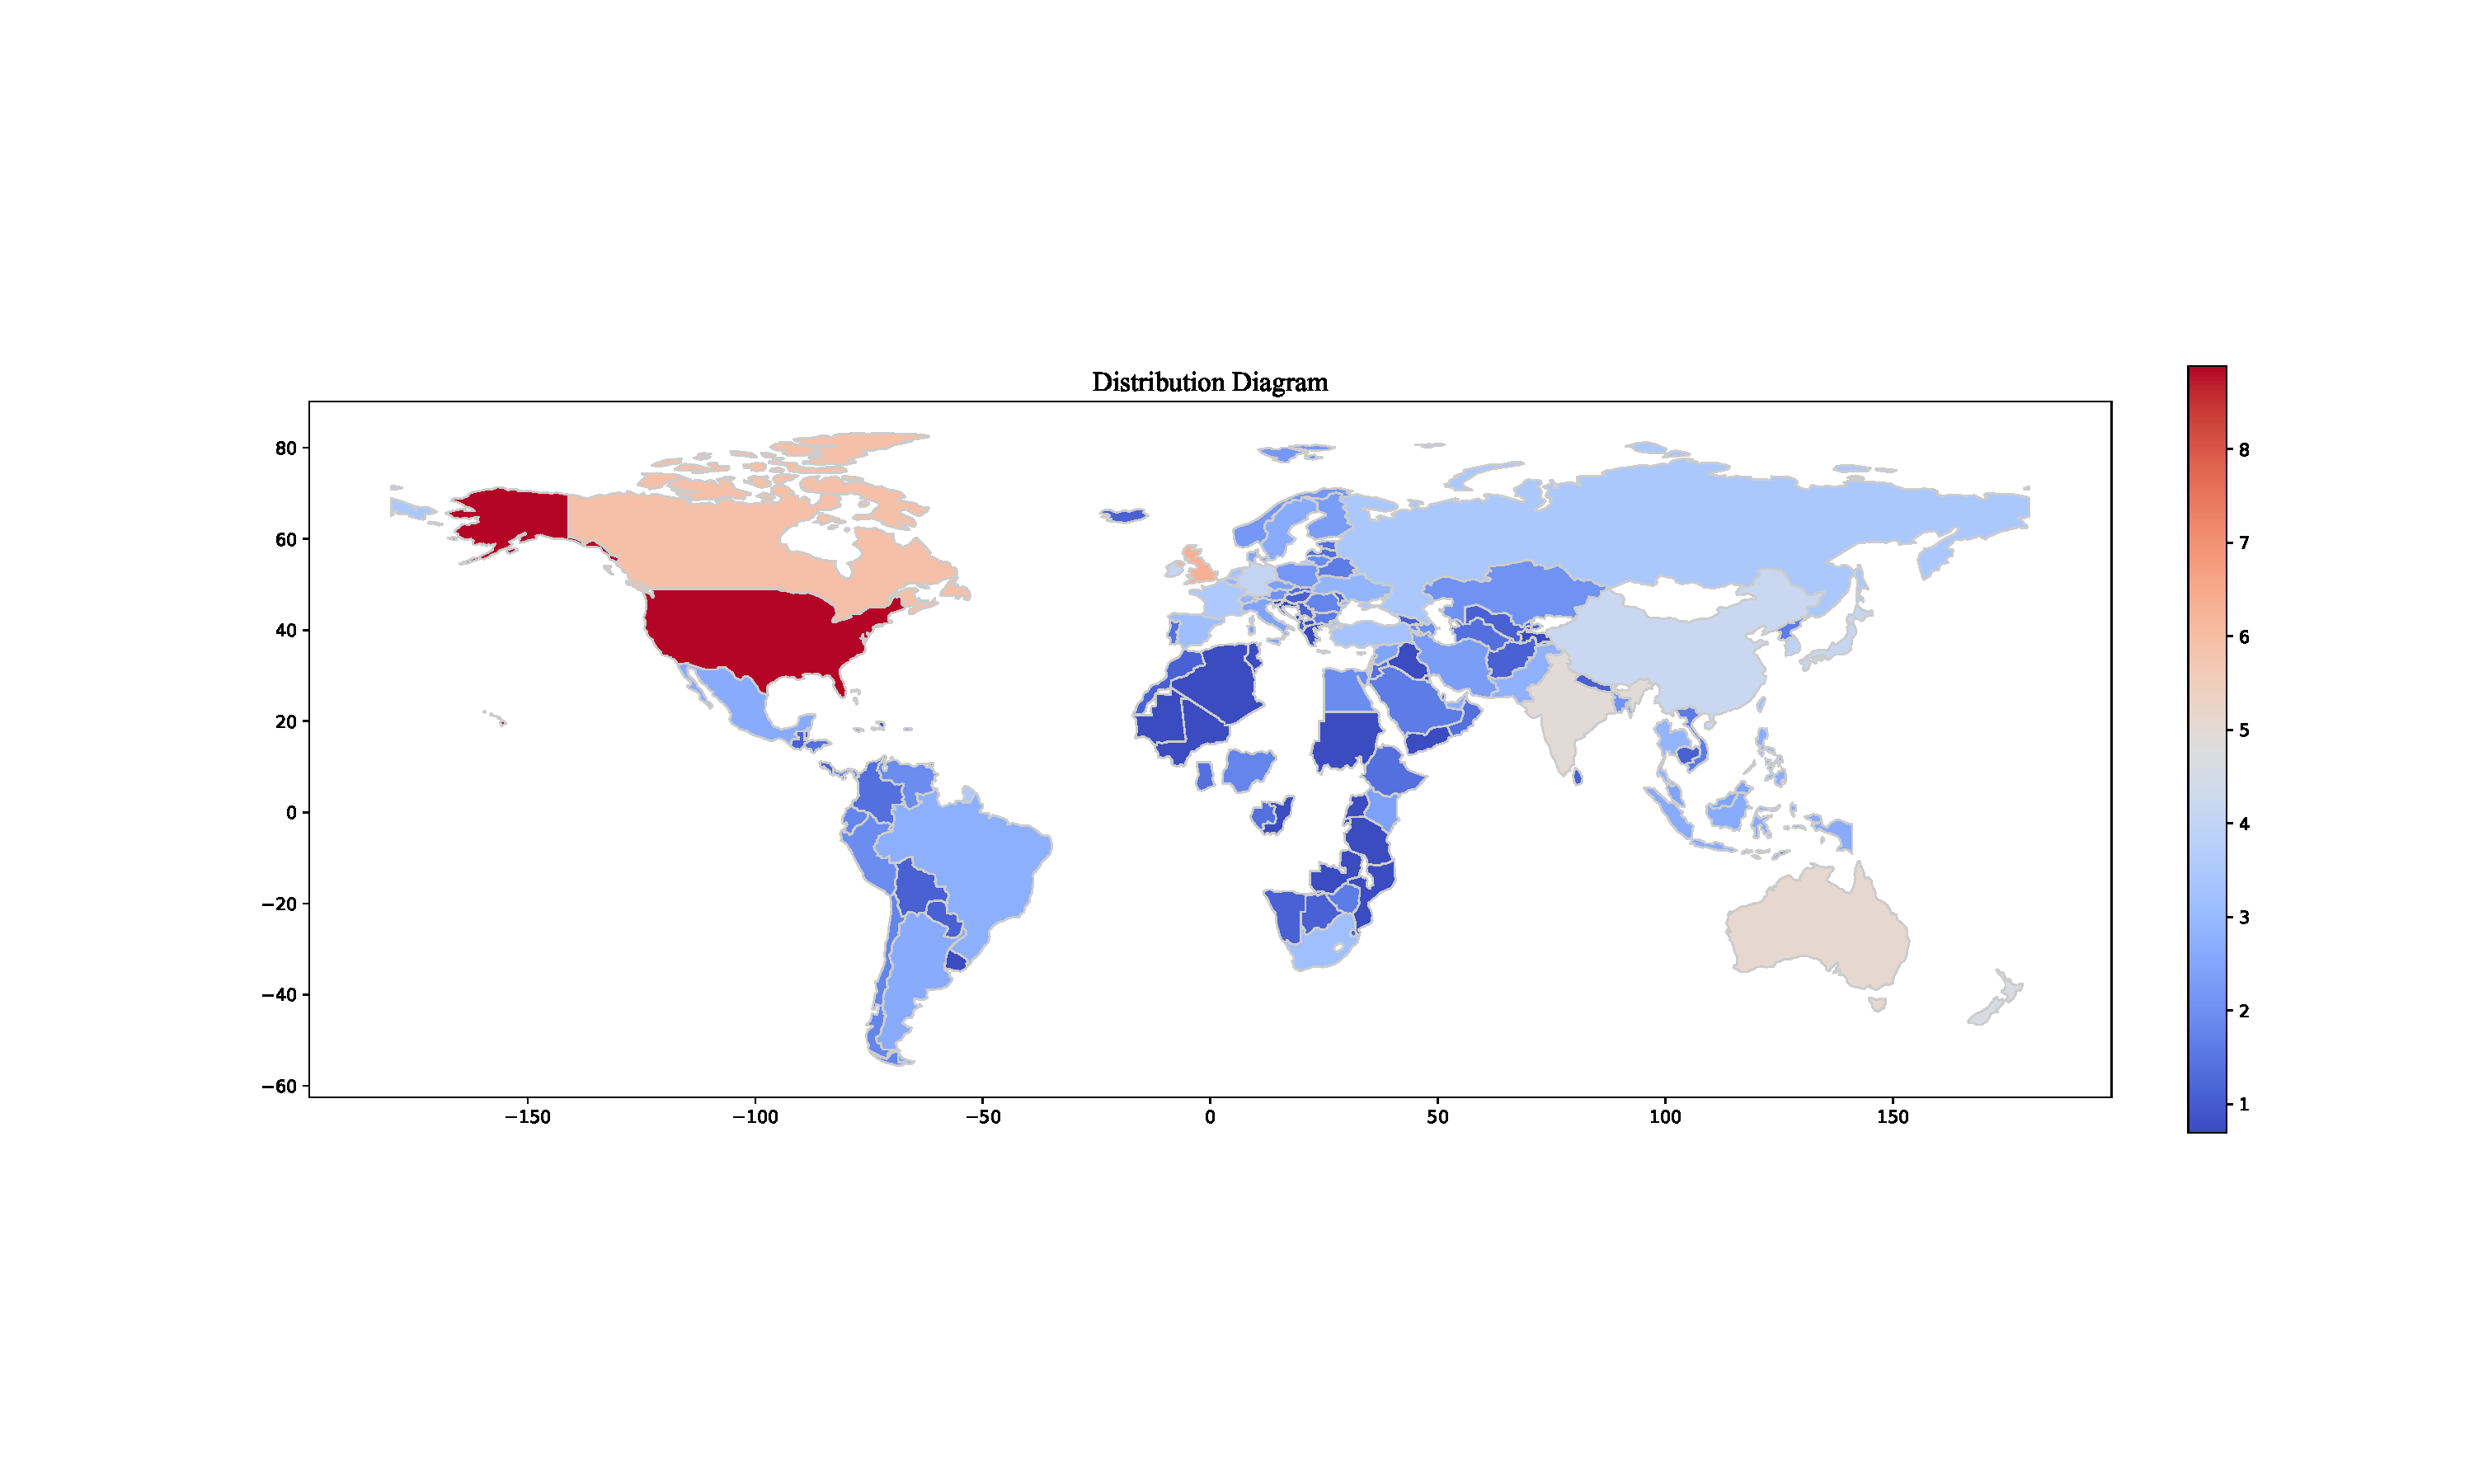
\includegraphics[width=1\linewidth]{../rsrc/distributions/Crime_distribution}
		\caption{Crime distribution}\label{fig:crime-distribution}
	\end{figure}
\subsection{High-prevalence regions}\label{subsec:high-prevalence-regions} %3.2
	We obtained population data $P_i$ for various countries over recent decades from the World Bank Group's website\cite{population}.
	Simultaneously, we processed data from the VCDB to tabulate the annual number of cybercrime incidents $D_i$ for each country from 2000 to 2025.
	However, due to discrepancies in the specific countries reported by the World Bank Group and those listed in the VCDB,
	we had to exclude certain countries to ensure that only those appearing in both datasets were retained.
	Ultimately, 109 countries were included in the model.
	To represent the average number of cybercrime incidents per capita,
	we calculated the ratio $D_i/P_i$ for each year from 2000 to 2025.
	Since the resulting values were too small for practical analysis,
	we scaled them by a factor of $10^{8}$ to express the data as the number of cybercrime incidents per 100 million people,
	denoted as $hmD/P_i$:
	\[ hmD/P_i = \frac{D_i}{P_i} \times 10^{8} \]

	According to the GCI (Global Cybersecurity Index) standards, countries are classified into five tiers, denoted as T1 to T5.
	We used this classification as the basis for K-means clustering analysis,
	dividing the 109 countries into five groups based on the percentiles published on the GCI website:
	the top 10\%, the next 20\%, the following 25\%, the subsequent 25\%, and the bottom 20\%.
	For each group, the annual average of $hmD/P_i$ (the number of cybercrime incidents per 100 million people) was calculated.
	To visualize the results, we constructed a 3D clustering heatmap of cybercrime trends,
	where the x-axis represents the five tiers (T1 to T5),
	the y-axis represents the time span from 2000 to 2025,
	and the z-axis represents the average $hmD/P_i$ values.
	This visualization is presented in Figure\ref{fig:3D_with_Spaced_Projection}.
	\begin{figure}[htbp]
		\centering
		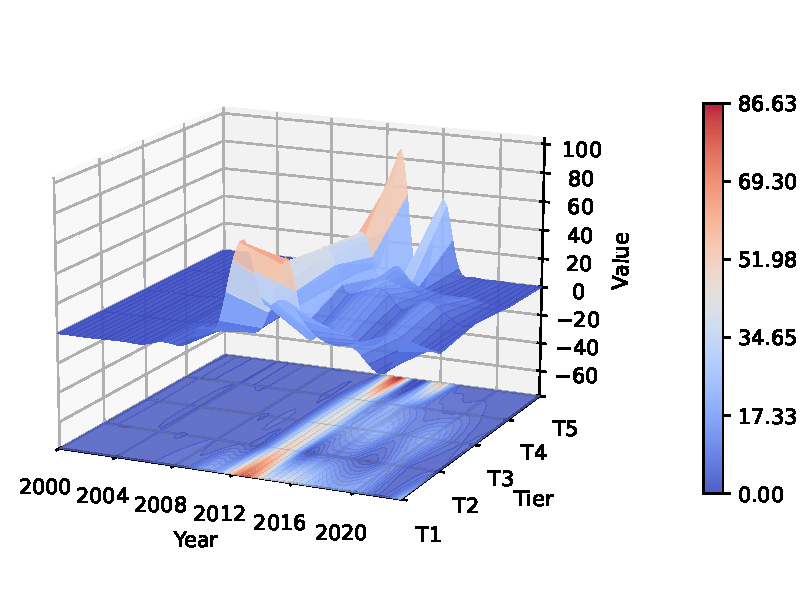
\includegraphics[width=0.8\linewidth]{../rsrc/distributions/3D_with_Spaced_Projection}
		\caption{3D with Spaced Projection}\label{fig:3D_with_Spaced_Projection}
	\end{figure}
\subsection{Other Cybercrime Incidents}\label{subsec:other-cybercrime-incedents} % 3.3
	Using additional data obtained from the VCDB,
	we constructed heatmaps on a global scale based on the number of successful cybercrimes, thwarted cybercrimes, and reported cybercrimes, respectively.
	Due to the disproportionately high volume of data from the United States,
	we applied the same logarithmic transformation (\( y = \log(1 + x) \)) as in Figure~\ref{fig:crime-distribution} for consistency,
	where $x$ represents successful attacks, thwarted attacks, and reported attacks,
	resulting in the three sub-figures presented in Figure\ref{fig:other-cybercrime-incidents}.

	In sub-figure (a), the number of successful attacks closely aligns with the total number of attacks in most countries.
	For instance, the United States recorded 7,189 successful attacks out of 7,236 total attacks,
	yielding a success rate of \( \frac{7189}{7236} \approx 99.35\% \).
	Similarly, the United Kingdom reported 569 successful attacks out of 574 total attacks,
	with a success rate of \( \frac{569}{574} \approx 99.13\% \).

	In contrast, countries with lower attack volumes did not show significant differences between the total number of attacks and the number of successful attacks,
	indicating that almost every attempted attack was successful.

	In sub-figure (b), only the United States and Canada reported thwarted attack cases, with 6 and 2 instances, respectively.

	In sub-figure (c), the number of successfully reported attacks and the number of countries involved were significantly higher than in sub-figure (b).
	This suggests that while many attacks were successful, a portion of them were detected and reported.
	\begin{figure}[htbp]
		\centering
		\subfloat[Successful Cybercrime Incidents]{
			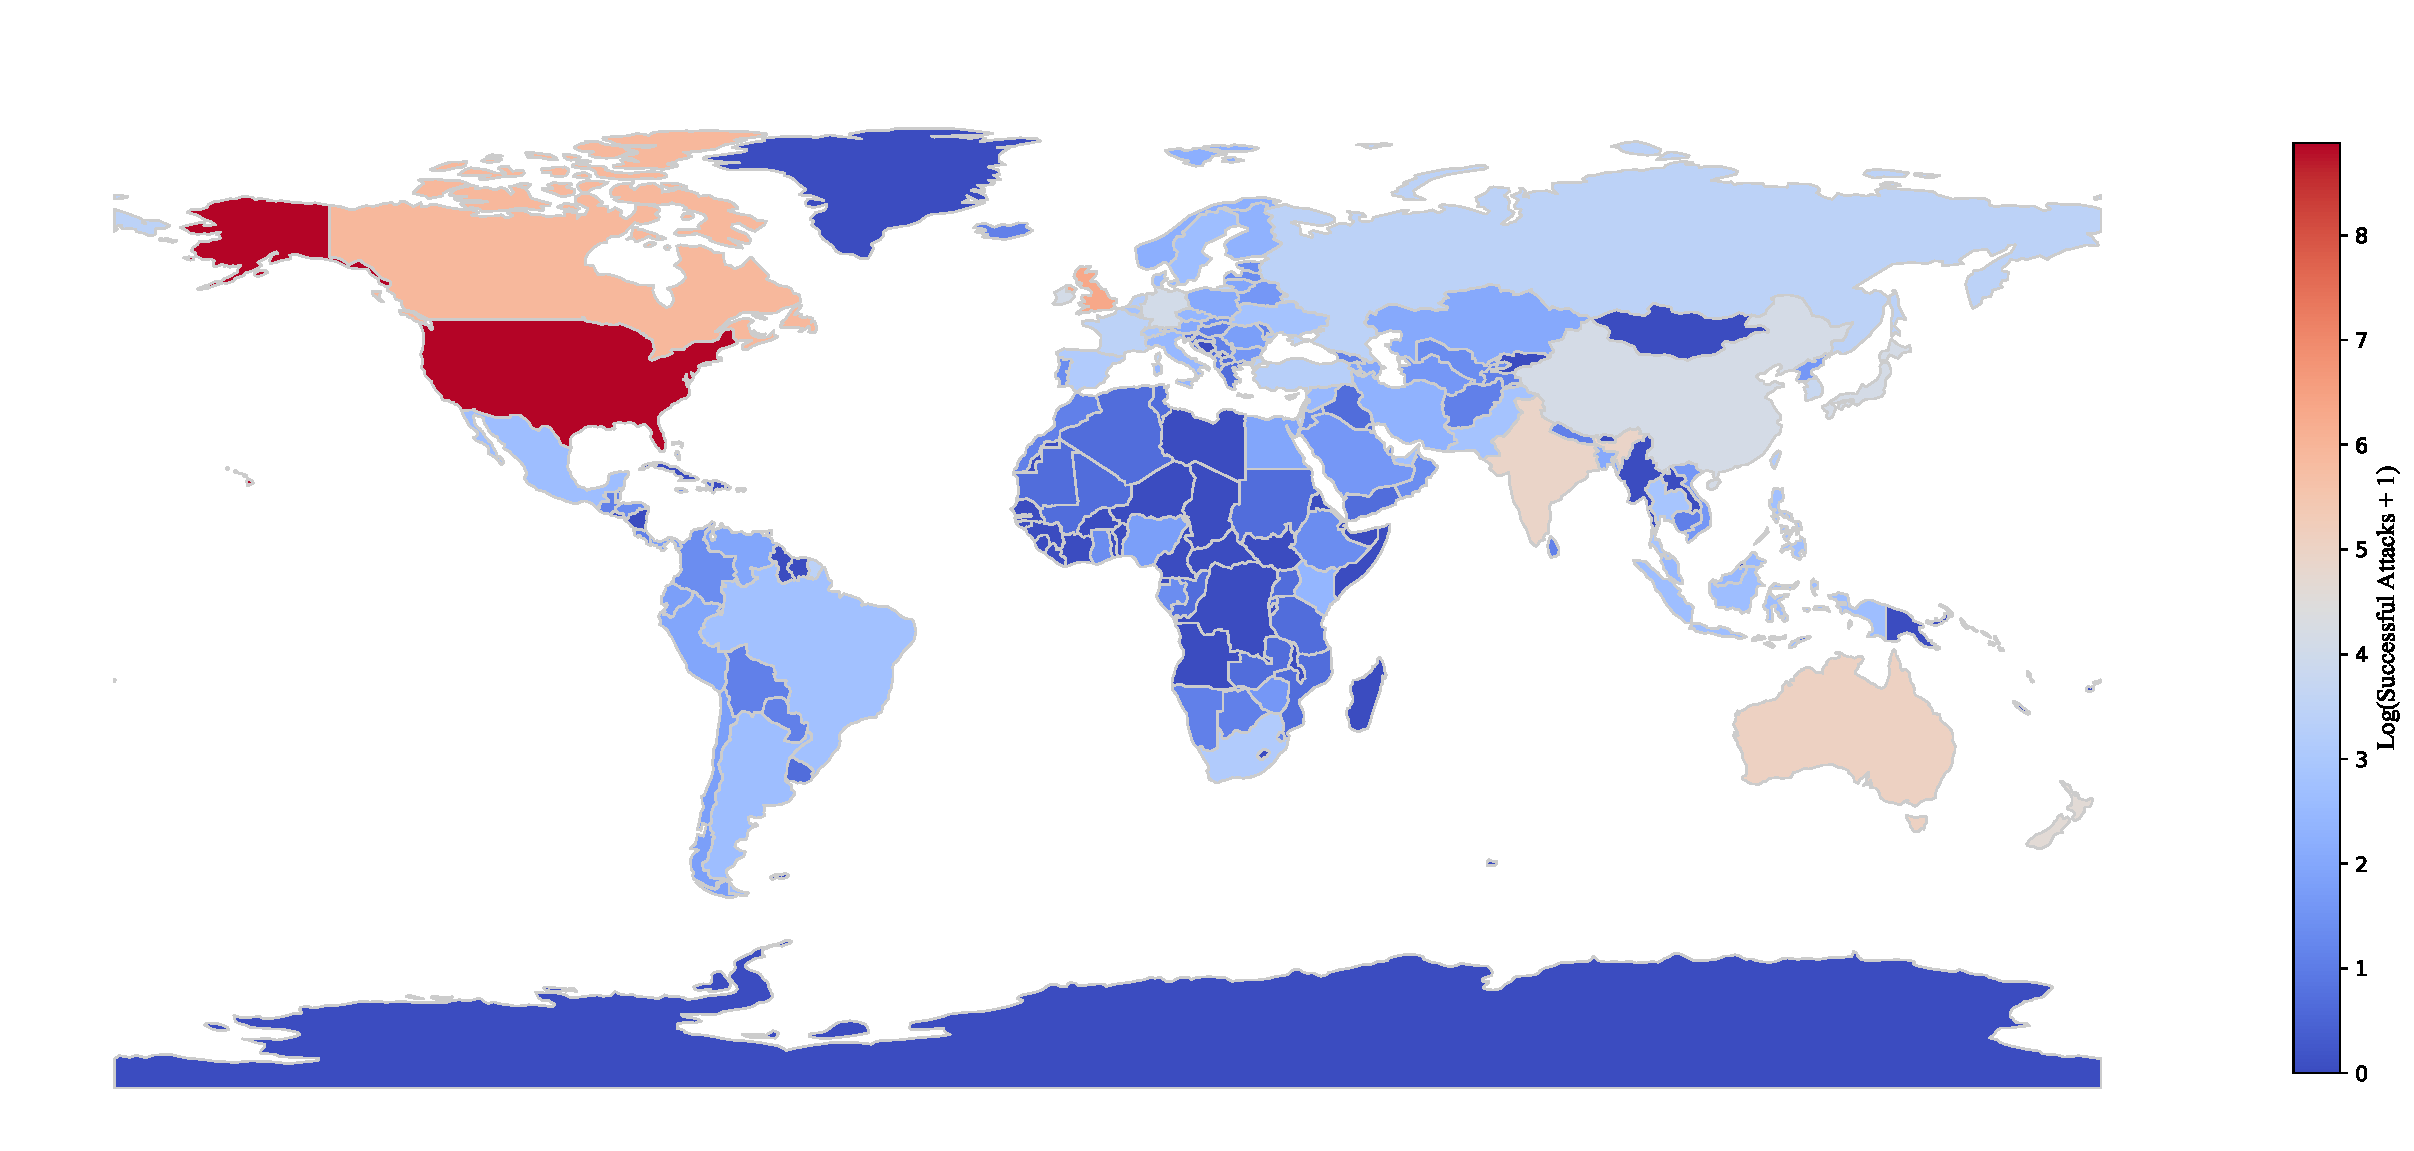
\includegraphics[width=0.8\linewidth]{../rsrc/distributions/Crime_Successful_distribution}
		}\\
		\subfloat[Mitigated Cybercrime Attempts]{
			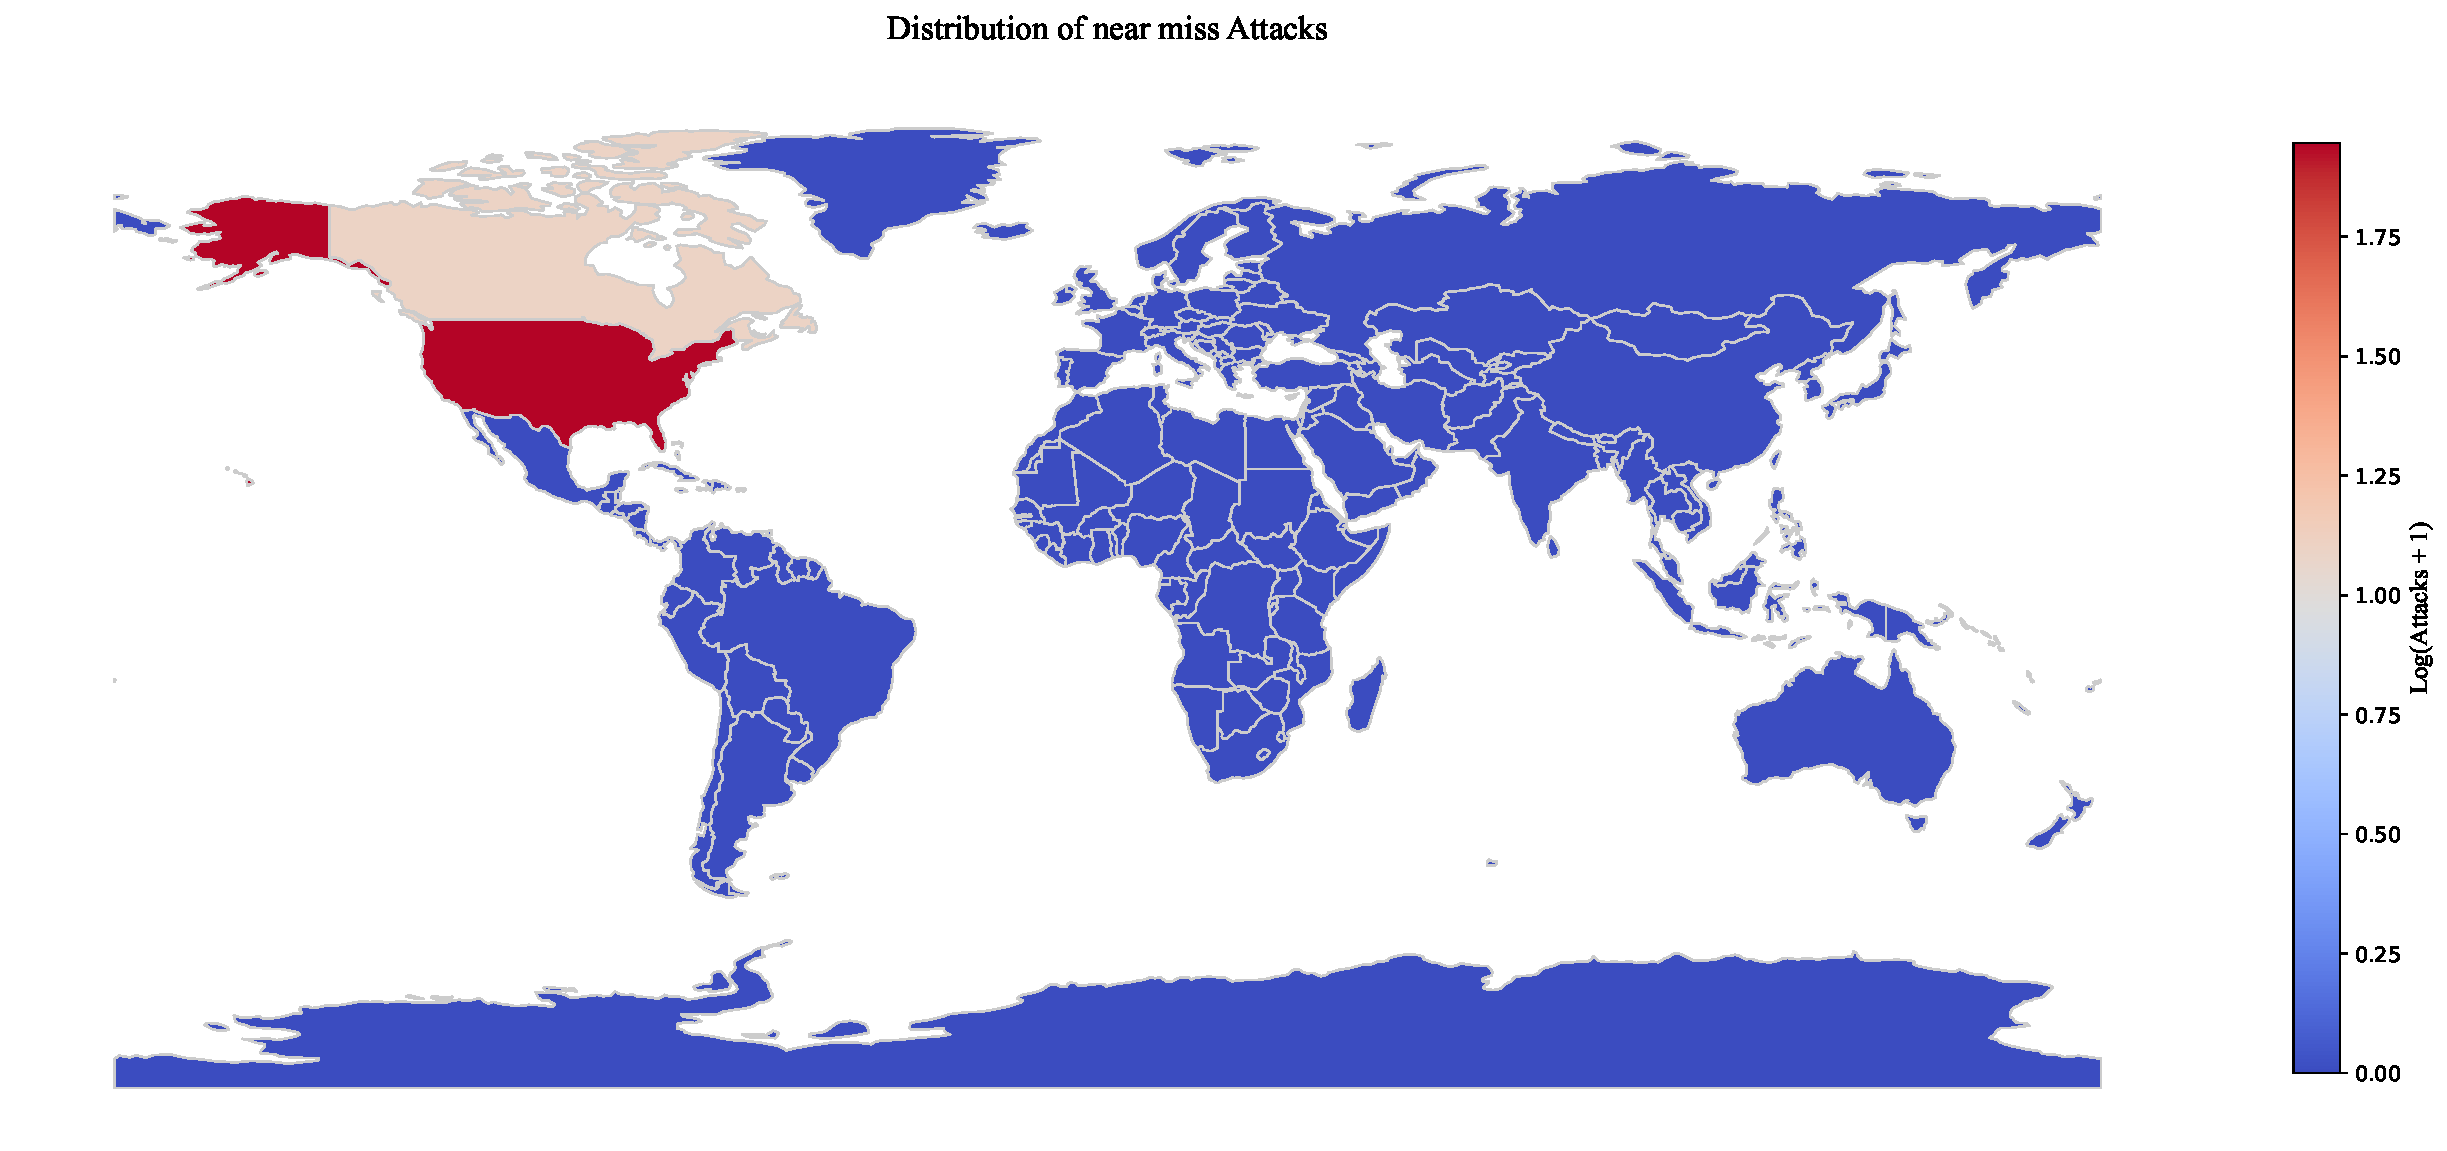
\includegraphics[width=0.4\linewidth]{../rsrc/distributions/Crime_NearMiss_distribution}
		}\hfill
		\subfloat[Reported Cybercrime Incidents]{
			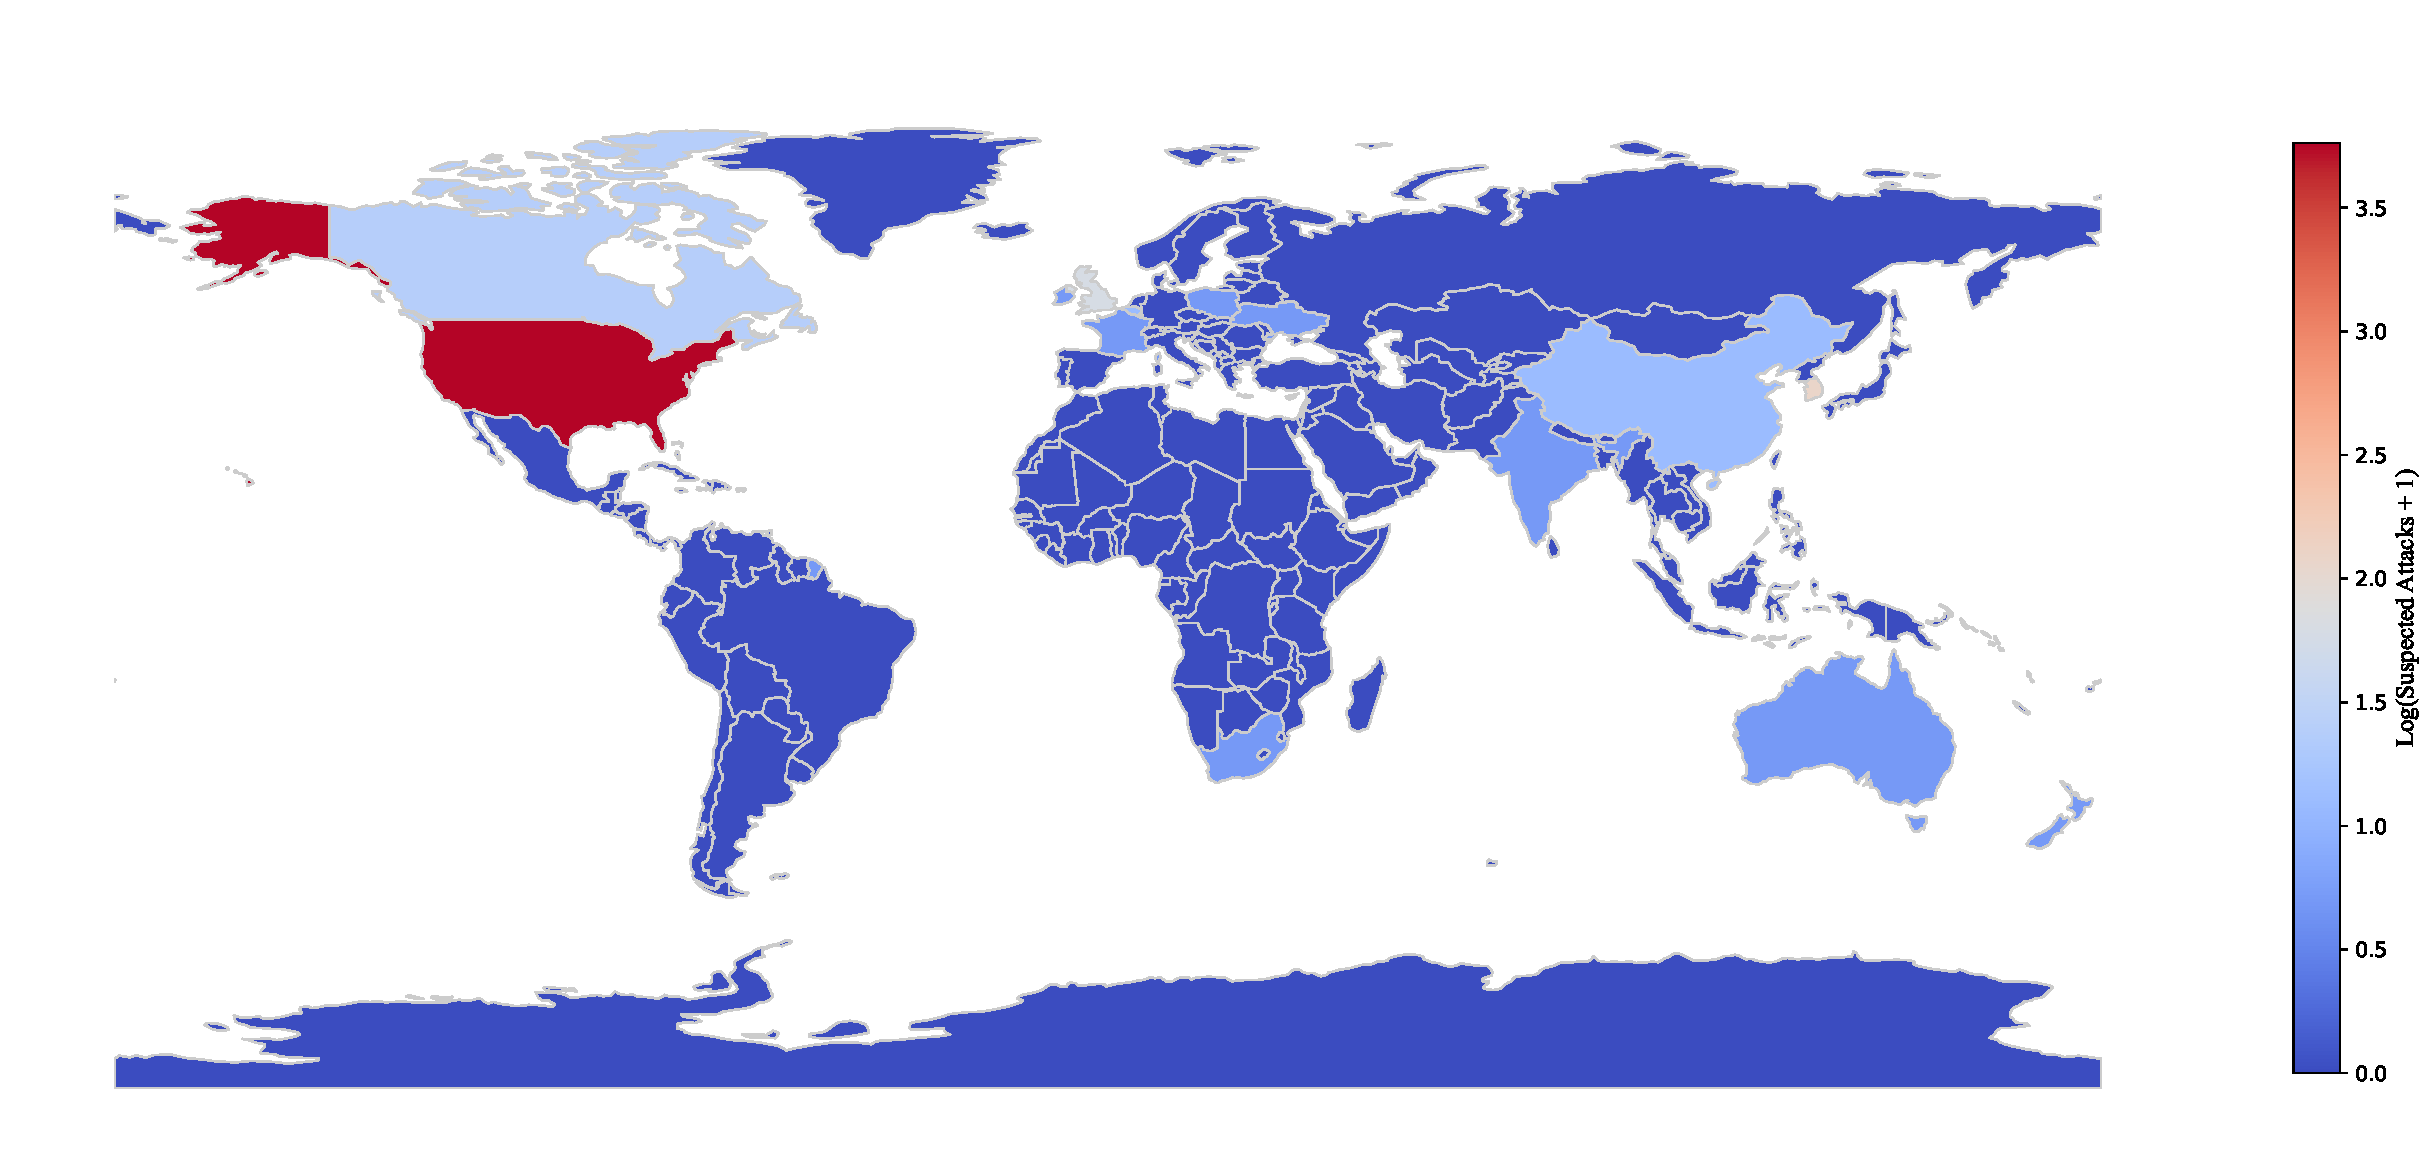
\includegraphics[width=0.4\linewidth]{../rsrc/distributions/Crime_Suspected_distribution}
		}\\
		\caption{Other Cybercrime Incidents}\label{fig:other-cybercrime-incidents}
	\end{figure}
\subsection{Pattern Discovery}\label{subsec:pattern-discovery} %3.4
	As illustrated in Figure~\ref{fig:other-cybercrime-incidents},
	the majority of countries worldwide lack adequate defensive capabilities against cyberattacks.
	Among the disclosed incidents, only the United States and Canada have recorded successful defense cases,
	with the United States reporting 6 instances and Canada reporting 2.
	This disparity can be attributed to the early development and technological maturity of the United States' cybersecurity infrastructure.
	The advanced technologies employed by both the U.S.\ government and private enterprises have enabled a certain level of resilience against some cyberattacks.
	Additionally, the disproportionately high volume of cybercrime in the United States plays a significant role.
	The extensive record of cyber incidents increases the likelihood of successful defenses,
	as it provides more opportunities for defensive mechanisms to be tested and refined.
	In contrast, other countries lack both the advanced defensive technologies and the high volume of cybercrime records that the United States possesses.
	Consequently, no successful defense cases have been reported for these countries in the VCDB .

	Cybercrime exhibits distinct patterns both across countries categorized by the GCI (Global Cybersecurity Index) and over time.
	To analyze these trends, we calculated the proportion of cybercrime incidents and visualized the results in Figure 2.
	This figure illustrates the annual average $hmD/P_i$ for each GCI tier (T1 to T5) from 2000 to 2025,
	providing a comprehensive overview of the spatial and temporal distribution of cybercrime.
	\begin{itemize}
		\item \textbf{2012 to 2016} Around 2012, both T5 and T1 countries exhibited the highest number of cybercrime incidents.
			Specifically, the $hmD/P_i$ index for T5 countries reached 86.63,
			marking the highest average number of cybercrime incidents among all tiers over the 25-year period.
			In contrast, T2, T3, and T4 countries reported significantly fewer incidents compared to T1 and T5 during this timeframe.
			The high cybercrime rates in T5 countries can be attributed to their poor performance across all five GCI assessment metrics:
			Legal, Technical, Organizational, Capacity Development, and Cooperation.
			These deficiencies likely contributed to their low GCI rankings and inadequate cybersecurity infrastructure,
			which in turn made them more vulnerable to cybercrime.
			On the other hand, T1 countries, despite their high GCI rankings, experienced a surge in cybercrime incidents around 2012.
			This suggests that even these nations were not fully prepared for the rapid evolution of cyber threats during this period.
			It is important to note that the fifth edition of the GCI assessment data was only released in 2024,
			meaning that the high rankings of T1 countries in 2024 do not necessarily reflect their cybersecurity capabilities in 2012.
		\item \textbf{2016 to 2020} During the period from 2016 to 2020, the number of cybercrime incidents declined across all tiers, from T1 to T5.
			Notably, T1 countries experienced a sharp decrease in cybercrime rates.
			This trend can be attributed to several factors.
			First, T1 countries, with their advanced technological infrastructure and robust cybersecurity policies,
			were better equipped to adapt to emerging threats.
			During this period, many T1 nations implemented comprehensive cybersecurity strategies,
			including stricter regulations, enhanced public-private partnerships, and increased investment in cybersecurity education and training.
			Additionally, international cooperation played a significant role in mitigating cross-border cyber threats.
			For example, initiatives such as information sharing through organizations like VERIS
			contributed to a more coordinated global response to cybercrime.
			However, despite the overall decline, T5 countries remained the most affected by cybercrime,
			likely due to their low performance in the GCI assessment metrics.
			These deficiencies continued to hinder their ability to build effective cybersecurity defenses,
			leaving them more vulnerable to cyber threats.
		\item \textbf{2020 till Present} Around 2020, a remarkable shift has occurred in the distribution of cybercrime incidents across the GCI tiers.
			Notably, the number of reported cybercrime incidents in T5 countries has dropped to almost negligible levels,
			a phenomenon that warrants further investigation.
			Similarly, T4 countries have maintained cybercrime rates comparable to those of T5.
			In contrast, T1, T2, and T3 countries continue to report a portion of cybercrime incidents,
			although these numbers have been steadily decreasing year by year.
			This trend may reflect the cumulative impact of sustained investments in cybersecurity infrastructure, policy improvements, and international collaboration among higher-tier countries.
			However, the sharp decline in T5 countries' cybercrime records remains puzzling and could be attributed to underreporting.
			Further research is needed to explore these potential explanations.
	\end{itemize}


\section{The establishment and solution of problem 2 model}\label{sec:the-establishment-and-solution-of-problem-2-model} %4
	\subsection{Shit, bro*2}\label{subsec:shit-bro*2} %4.1
	
\section{The establishment and solution of problem 3 model}\label{sec:the-establishment-and-solution-of-problem-3-model} %5
	\subsection{Shit, bro*3}\label{subsec:shit-bro*3} %5.1
	
\section{Future expected data}\label{sec:future-expected-data} %6

\section{Advantages \& Disadvantages}\label{sec:advantages-&-disadvantages} %7

\bibliographystyle{plain}
\bibliography{references} %8

\section*{Appendix}\label{sec:appendix} %9


\end{document}